% !TEX root = ../main.tex

% Indicate the main file. Must go at the beginning of the file.

%-------------------------------------------------------------------------------
% CHAPTER TEMPLATE
%-------------------------------------------------------------------------------


\chapter{Theoretische Grundlagen} % Main chapter title
\label{Chapter2TheoretischeGrundlagen} % Change X to a consecutive number; for referencing this chapter elsewhere, use \ref{ChapterX}

Der Multifunction Vehicle Bus (nachvolgend als MVB abgekürtzt), ist ein in der Bahnindustrie verbreiteter Fahrzeugbus, welcher auf dem Prinzip \textit{single master - multiple slaves} aufbaut. In folgenden Abschnitten werden die Grundlagen des Bus sowie recherchierte Sniffer aufgezeigt.

%--------------------------------------------------------------------------------
% SECTION "Multifunction Vehicle Bus"
%--------------------------------------------------------------------------------

\section{Multifunction Vehicle Bus}

\textcolor{red}{Einführung in Grundbegriffe und das Konzept MVB, In der Regel ist zumindest ein kurzes Theoriekapitel notwendig. Es nimmt Bezug  auf das thematische Oberthema, aber natürlich nicht auf allgemeine theoretische Grundlagen etwa aus der Naturwissenschaft.}

Der Abschnitt beleuchtet die wesentlichen Aspekte des Physical und Link Layers des Datenbusses gemäß der Norm SN EN 61375. Der Fokus liegt auf der Datenübertragungsgeschwindigkeit, Bit-Encoding und den Steuermechanismen wie den Startdelimitern und dem Master-Slave-Prinzip. Neben den technischen Grundlagen, wie der Manchester-Kodierung und den Non-Data-Symbolen, wird die Struktur von Frames und Telegrammen detailliert beschrieben. Dadurch wird die Grundlage geschaffen, um die Herausforderungen in der Entwicklung nachvollziehen zu können.


%-----------------------------------
% SUBSECTION "MVB Bus"
%-----------------------------------

%\textcolor{red}{MVB Aufbau, Master Slave Prinzip, Telegrammme, F-Codes}


\subsection{Physical Layer - Geschwindigkeit auf dem Datenbus}
Die "'Signalling speed"' ist in der Norm \textit{SN EN 61375-3-1:2012 Kap. 4.3.1} definiert. Diese lautet 1.5 Mbit/s $\pm$ 0.01\% mit Manchester Encoding (siehe \ref{subsub:BitEncoding})

\begin{itemize}
  \item BR (Bit rate): 1.5 MHz oder 1.5 Mbit/s
  \item BT (Bit time): 666.7 ns
\end{itemize}

\subsection{Physical Layer - Bit Encoding}
\label{subsub:BitEncoding}
Die Frame-Data sollen gemäss folgender \textit{Bit Encoding} (Abb. \ref{fig:manchester_Bit_Encoding}) kodiert werden.

\begin{itemize}
    \item Eine "'1"' soll kodiert werden als ein \textbf{HIGH} in der ersten und dann ein \textbf{LOW} in der zweiten Hälfte der 1,0 BT
    \item Eine "'0"' soll kodiert werden als ein \textbf{LOW} in der ersten und dann ein \textbf{HIGH} in der zweiten Hälfte der 1,0 BT
\end{itemize}

\begin{figure}[h!]
    \centering
    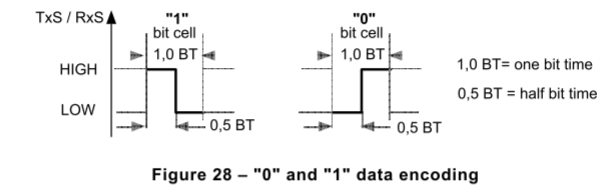
\includegraphics[width = 0.7 \textwidth]{Figures/Chap2/Grundlagen/MVB_DOKU/Layer/Bit_Encoding.png}
    \caption{Machester Bit encoding}
    \label{fig:manchester_Bit_Encoding}
\end{figure}

\subsection{Physical Layer - Non Data Symbols} 
\label{subsub:NonDataSymbols}
Der Start-Delimiter enthält \textit{Non Data Symbols}, welche zur Synchronisierung verwendet werden. Diese Symbols werden ebenfalls \textit{Manchastercode violations} genannt. Folgende Liste zeigt, wie die Symbols (Abb. \ref{fig:NonDataSymbolsEncoding}) kodiert sind

\begin{itemize}
    \item "'NH"' soll kodiert werden als ein \textbf{HIGH} Singal während einer Priode von 1,0 
    \item "'NL"' soll kodiert werden als ein \textbf{LOW} Singal während einer Priode von 1,0 BT
\end{itemize}

\begin{figure}[h!]
    \centering
    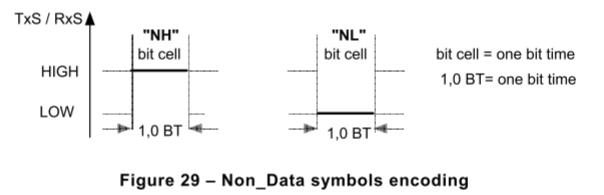
\includegraphics[width = 0.7 \textwidth]{Figures/Chap2/Grundlagen/MVB_DOKU/Layer/Non_Data_Symbol.png}
    \caption{Non Data Symbols encoding}
    \label{fig:NonDataSymbolsEncoding}
\end{figure}

\subsection{Physical Layer - Start Delimiter}
Der Startdelimiter hat die Funktion ein Frame eindeutig zu identifizieren. Hierbei gibt es zwei unterscheidbare Startdelimiter, der \textit{Master Frame Delimiter} und der \textit{Slave Frame Delimiter}. In Abbildung \ref{fig:FrameDelimiterMasterSlave} sind beide Start Delimter aufgezeigt. Gut zu sehen sind die in Kapitel \ref{subsub:NonDataSymbols} erwähnten Manchester Violations. 

\begin{figure}[h!]
    \centering
    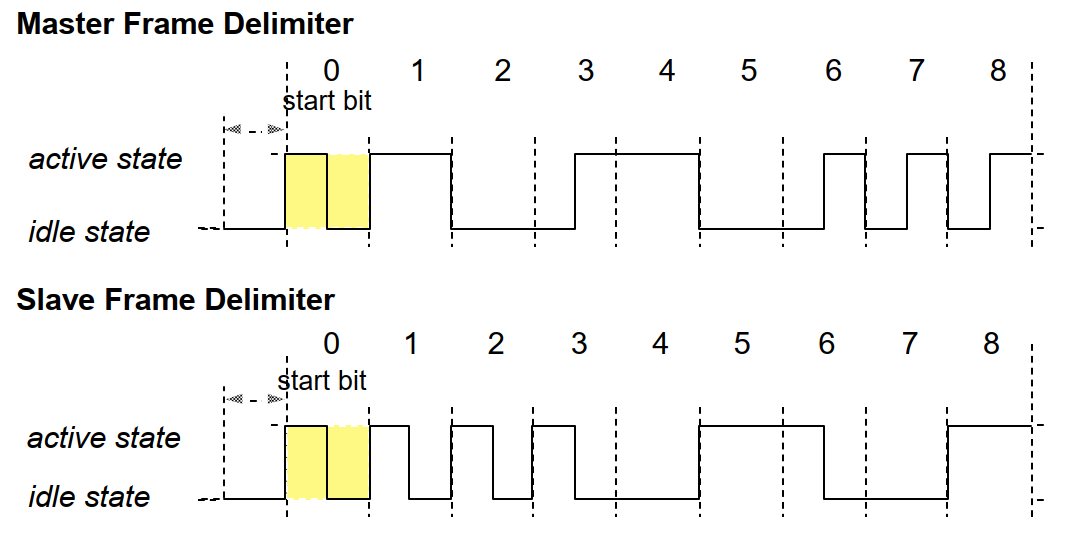
\includegraphics[width=0.8\linewidth]{Figures/Chap2/Grundlagen/MVB_DOKU/Layer/Frame_Delimiter.png}
    \caption{Caption}
    \label{fig:FrameDelimiterMasterSlave}
\end{figure}

\subsection{Link Layer - Master / Slave Prinzip}
Die Echtzeit des MVB wird durch ein Master - Slave Prinzip realisiert. Der Master fordert mit einem definierten \textit{Master\_Frame} die Daten der jeweiligen Slave-Teilnehmer an. Der Slave beantwortet die Anfrage mit einem \textit{Slave\_Frame}. Das Master- und Slave-Frame bilden zusammen ein Telegram (Siehe Abbildung \ref{fig:Fig39_Telegamm_definition.png}). 

\begin{figure}[h!]
    \centering
    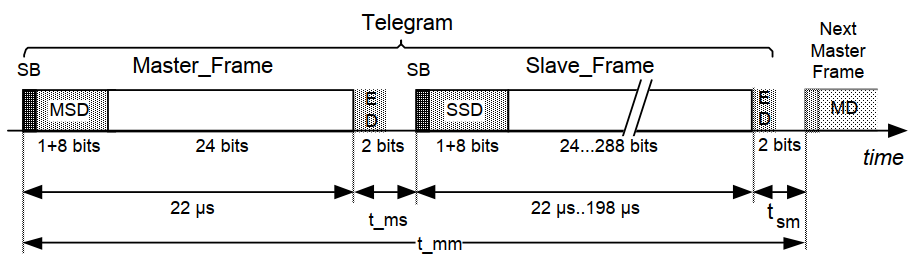
\includegraphics[width=0.85\linewidth]{Figures/Chap2/Grundlagen/MVB_DOKU/Frames und Telegramme/Fig39_Telegamm_definition.png}
    \caption{Master- und Slave-Frame bilden ein Telegram}
    \label{fig:Fig39_Telegamm_definition.png}
\end{figure}

In der Norm \textit{SN EN 61375} sind die Telegramme in 16 verschiedene F-Codes (Frame-Codes) unterteilt. In Abbildung \ref{fig:FCodeListe} ist eine tabellarische Auflistung zu sehen. 

\begin{figure}[h!]
    \centering
    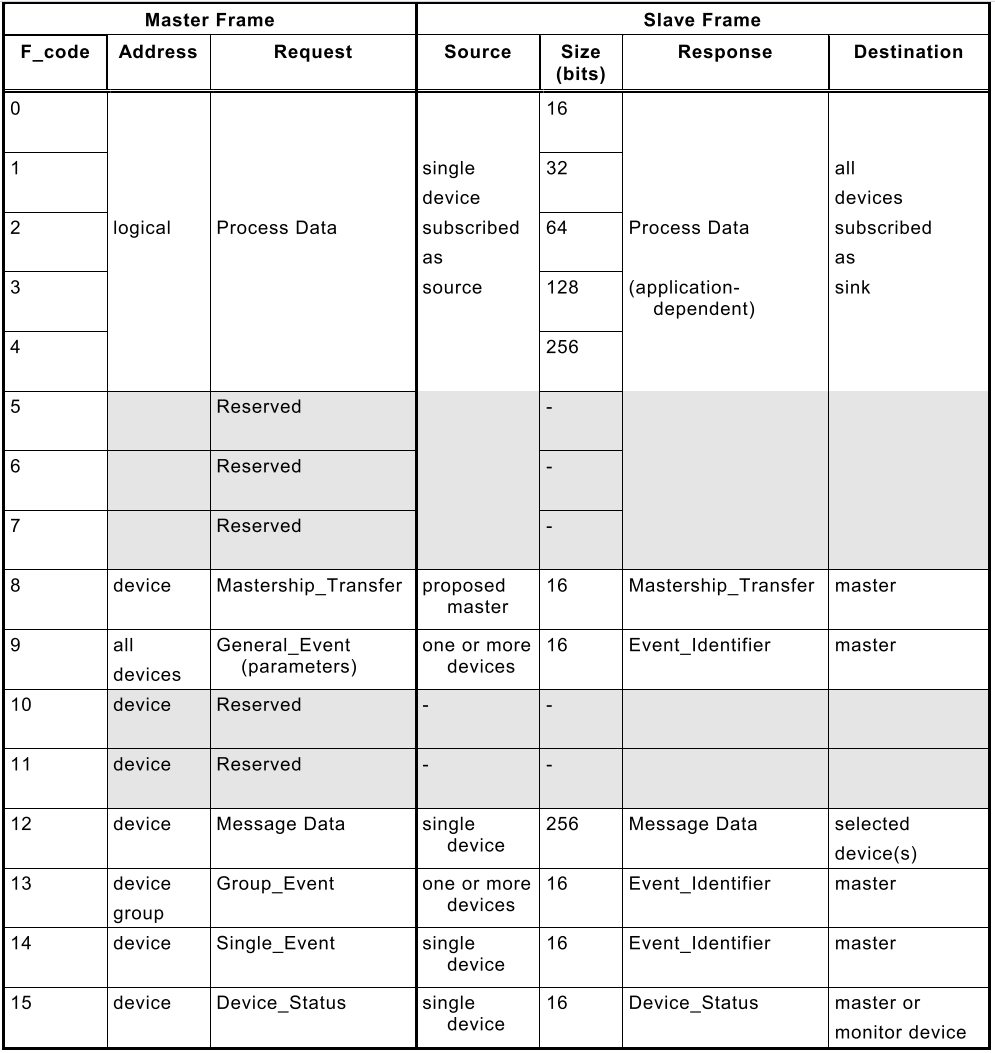
\includegraphics[width=0.8\linewidth]{Figures/Chap2/Grundlagen/MVB_DOKU/Frames und Telegramme/F-Code Liste.png}
    \caption{Caption}
    \label{fig:FCodeListe}
\end{figure}

\newpage

\subsection{Linklayer - Master Frame}
Das Master-Frame ist der Anfang eines Telegrames und wird immer vom Busmaster gesendet. Die ersten 8 Bits entsprechen dem Master Frame Delimiter in Abbildung \ref{fig:FrameDelimiterMasterSlave}. 

\begin{figure}[h!]
    \centering
    \begin{minipage}{0.33 \textwidth}
        \centering
        \begin{enumerate}
            \item Master Start Delimiter
            \item 16 Bit Frame Data
            \begin{enumerate}
                \item F-Code: 4 Bit
                \item Data: 12 Bit
            \end{enumerate}
            \item 8 bit check sequenze 
            \item End Delimiter
        \end{enumerate}
    \end{minipage}
    \hfill
    \begin{minipage}{0.65 \textwidth}
        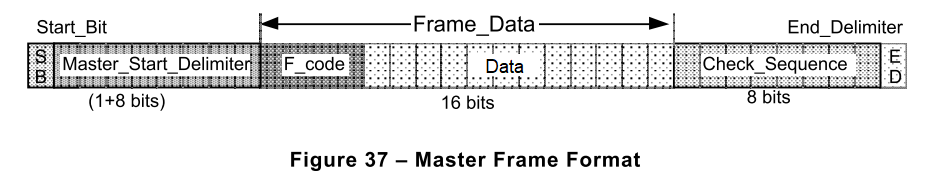
\includegraphics[width = \textwidth]{Figures/Chap2/Grundlagen/MVB_DOKU/Frames und Telegramme/Fig37_MasterFrameFormat.png}
        \caption{Master Frame Format}
        \label{fig:MasterFrameFormat}
    \end{minipage}
        
\end{figure}

\subsection{Linkayer - Slave Frame}
Das Slave Frame folgt direkt nach dem Master Framer, sofern der angesprochene Slave eingeschalten und sendefähig ist. Ansonsten würde der Master nach einer definierten maximalen Wartezeit ein neues Telegramm beginnen. \newline
Im Gegensatz zum Masterframe hat der Slave Frame verschiedene längen, je nach F-Code. Je nach grösse werden ebenfalls mehrere Check-Sequenzen geschickt. Eine Check-Sequrnz kann dabei bis zu 64 Bits verifizieren.

\begin{enumerate}
    \item Slave Start Delimiter (8 bit)
    \item 16 - 256 bit Frame Data (individuell)
    \item Check sequence nach maximal 64bit Daten 
    \item End Delimiter
\end{enumerate}

\begin{figure}[h!]
    \centering
    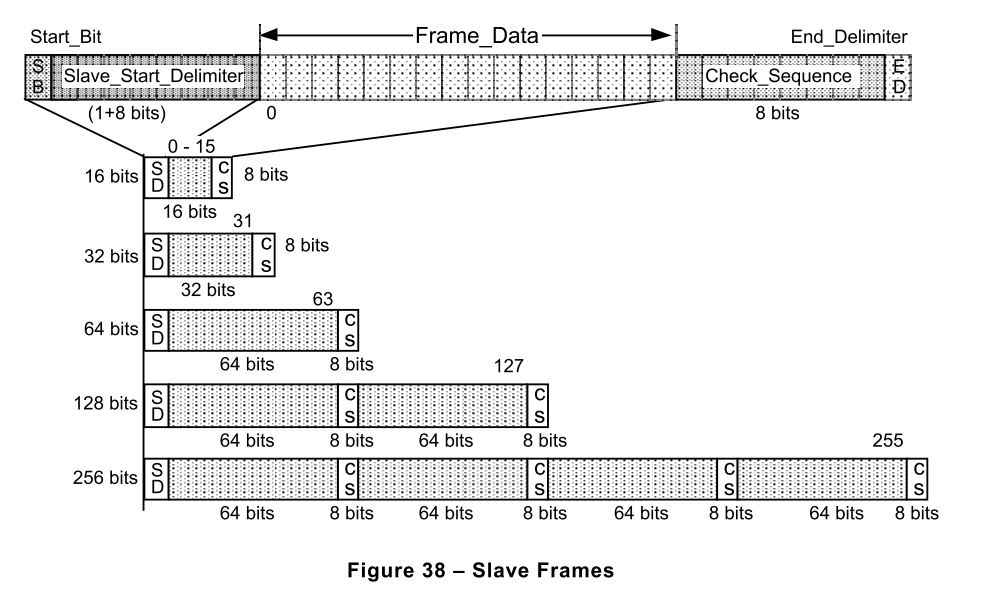
\includegraphics[width = 0.8 \textwidth]{Figures/Chap2/Grundlagen/MVB_DOKU/Frames und Telegramme/Fig38_SlaveFrameFormat.png}
    \caption{Slave Frame Format}
    \label{fig:SlaveFrameFormat}
\end{figure}
\newpage

\subsection{Linklayer - Check Sequence}
Die Prüfsequenz wird als zyklische Redundanzprüfung (CRC) für die 16, 32 oder 64 Bits an Daten berechnet, welche gemäss dem generativen Polynom in Gleichung \ref{equ:GenerativesPolynom} berechnet werden soll.

\begin{equation}
    G(x) = x^7 + x^6 + x^5 + x^2 + 1
    \label{equ:GenerativesPolynom}
\end{equation}

%-----------------------------------
% SUBSECTION "Sniffer"
%-----------------------------------

\section{Sniffer Device}
\textcolor{red}{Was ist ein Sniffer, was macht den Unterschied aus}


%--------------------------------------------------------------------------------
% SECTION Stand von Konkurenzprodukten
%--------------------------------------------------------------------------------

\section{Recherche bestehende Produkte}

%-----------------------------------
% SUBSECTION "Amit"
%-----------------------------------

\subsection{Konkurenz 1 (Amit Transportation)}
\textcolor{red}{Amit MVB Analyzer}


%-----------------------------------
% SUBSECTION "Ci4Rail"
%-----------------------------------

\subsection{Konkurenz 2 (Ci4Rail)}
\textcolor{red}{IP\ Based\ Sniffer}


%-----------------------------------
% SUBSECTION "Yacer"
%-----------------------------------

\subsection{Konkurenz 3 (Yacer MVB-Analyzer Protocol Analyzer)}
\textcolor{red}{Ebenfalls IP Based}


%-----------------------------------
% SUBSECTION "Abgrenzung"
%-----------------------------------

\subsection{Angrenzung zu den bestehenden Produkten}
\textcolor{red}{Was macht unser Sniffer anders/ besser}


